\documentclass[aspectratio=169]{beamer}

\usetheme{Madrid}
\usecolortheme{default}

\usepackage{amsmath}
\usepackage{graphicx}
\usepackage{booktabs}
\usepackage{listings}
\usepackage{xcolor}

\definecolor{codegray}{RGB}{245,245,245}
\definecolor{codeblue}{RGB}{30,80,140}

\lstset{
  basicstyle=\ttfamily\small,
  backgroundcolor=\color{codegray},
  keywordstyle=\color{codeblue},
  columns=fullflexible,
  keepspaces=true,
  showstringspaces=false,
  frame=single
}

\setbeamertemplate{navigation symbols}{}
\setbeamertemplate{footline}{
  \hfill
  \usebeamerfont{page number in head/foot}
  \insertframenumber{} / \inserttotalframenumber
  \hspace{0.4cm}
  \vspace{0.25cm}
}

\title{CARD: Correlation Aware Restoration with Diffusion}
\author{Hadi Fathipour}
\date{Tir 1405 (June 2025)}

\begin{document}

\begin{frame}
  \centering
  
\includegraphics[width=1.8cm]{logo.png}

  \vspace{0.25cm}
  {\large\textbf{Research Project \(\cdot\) Digital image processing course}}

  \vspace{0.35cm}
  {\Large\textbf{CARD: Correlation Aware Restoration with Diffusion}}

  \vspace{0.2cm}
  \rule{0.78\textwidth}{0.4pt}

  \vspace{0.45cm}
  \begin{tabular}{rl}
    \textbf{Supervisor:} & Hossein ali Ghiassi rad \\
    \textbf{Student:} & Hadi Fathipour -- Student ID: 40411334 \\
    \textbf{Presentation Date:} & Tir 1405 (June 2025) \\
  \end{tabular}
\end{frame}

\begin{frame}{Motivation}
  Most image restoration methods assume image noise is independent and identically
  distributed Gaussian noise.

  \vspace{0.4cm}
  Real camera sensors, especially rolling-shutter CMOS sensors, can produce
  spatially correlated noise:
  \begin{itemize}
    \item neighboring pixels are statistically coupled;
    \item row-wise readout can create banding artifacts;
    \item restoration methods that ignore this structure can leave artifacts or over-smooth details.
  \end{itemize}
\end{frame}

\begin{frame}{Original CARD Paper}
  The paper proposes \textbf{CARD: Correlation Aware Restoration with Diffusion}.

  \vspace{0.3cm}
  Its main idea is:
  \[
    y = Hx_0 + n,
    \qquad
    n \sim \mathcal{N}(0, \sigma_y^2 \Sigma)
  \]

  \vspace{0.2cm}
  CARD whitens the measurement:
  \[
    \tilde{y} = \Sigma^{-1/2} y,
    \qquad
    \tilde{H} = \Sigma^{-1/2} H
  \]

  After whitening:
  \[
    \tilde{n} \sim \mathcal{N}(0, \sigma_y^2 I)
  \]

  This lets DDRM-style diffusion restoration operate under its usual i.i.d. noise assumption.
\end{frame}

\begin{frame}{What This Project Implements}
  This project implements a compact, CPU-friendly version of the CARD idea.

  \begin{itemize}
    \item Generate a synthetic test image.
    \item Build rolling-shutter-like correlated Gaussian noise.
    \item Construct a patch-local covariance matrix.
    \item Use covariance coloring to add correlated noise.
    \item Use covariance eigenbasis / whitening logic for restoration.
    \item Compare against a Gaussian denoising baseline.
  \end{itemize}

  \vspace{0.3cm}
  The implementation package is named \texttt{card}.
\end{frame}

\begin{frame}{Pipeline}
  \begin{enumerate}
    \item Create a clean image.
    \item Build covariance matrix \(\Sigma\).
    \item Generate correlated noise using a coloring matrix.
    \item Add noise to the image.
    \item Restore using:
      \begin{itemize}
        \item Gaussian baseline;
        \item CARD covariance-aware Wiener restoration.
      \end{itemize}
    \item Report PSNR and SSIM.
    \item Save visual output to \texttt{results/card\_demo.png}.
  \end{enumerate}
\end{frame}

\begin{frame}{Covariance Model}
  The project models local spatial correlation inside each patch.

  \[
    \Sigma_{ij}
    =
    \rho^{|r_i-r_j|}
    (0.45\rho)^{|c_i-c_j|}
    +
    \epsilon I
  \]

  \begin{itemize}
    \item \(r_i, c_i\): row and column coordinates of pixel \(i\) in a patch.
    \item \(\rho\): correlation strength.
    \item \(\epsilon I\): small regularization for numerical stability.
  \end{itemize}

  This creates stronger row-wise correlation, similar to rolling-shutter artifacts.
\end{frame}

\begin{frame}{Noise Coloring and Whitening}
  The covariance matrix is decomposed with eigenvalue decomposition:
  \[
    \Sigma = Q \Lambda Q^T
  \]

  Coloring matrix:
  \[
    C = Q \Lambda^{1/2} Q^T
  \]

  Whitening matrix:
  \[
    W = Q \Lambda^{-1/2} Q^T
  \]

  \begin{itemize}
    \item Coloring transforms i.i.d. Gaussian noise into correlated noise.
    \item Whitening transforms correlated noise toward an i.i.d. form.
  \end{itemize}
\end{frame}

\begin{frame}[fragile]{Main Run Command}
  The project is reproducible with \texttt{uv}.

  \begin{lstlisting}[language=bash]
uv sync
uv run python main.py
  \end{lstlisting}

  Verification:

  \begin{lstlisting}[language=bash]
uv run pytest
uv run ruff check .
uv run basedpyright
  \end{lstlisting}
\end{frame}

\begin{frame}{Implementation Structure}
  \begin{table}
    \centering
    \begin{tabular}{ll}
      \toprule
      File & Responsibility \\
      \midrule
      \texttt{card/noise.py} & covariance, coloring, whitening, noise generation \\
      \texttt{card/restoration.py} & Gaussian baseline and CARD restoration \\
      \texttt{card/metrics.py} & PSNR and SSIM metrics \\
      \texttt{card/images.py} & synthetic image and output image grid \\
      \texttt{card/pipeline.py} & end-to-end experiment pipeline \\
      \texttt{main.py} & command-line entry point \\
      \bottomrule
    \end{tabular}
  \end{table}
\end{frame}

\begin{frame}{CARD Restoration}
  The restoration step uses the covariance eigenbasis.

  \begin{enumerate}
    \item Split the noisy image into patches.
    \item Project patch vectors into the covariance eigenbasis.
    \item Estimate signal variance and noise variance per component.
    \item Apply Wiener-style shrinkage:
      \[
        g_i = \frac{\sigma^2_{\text{signal}, i}}
        {\sigma^2_{\text{signal}, i} + \sigma^2_{\text{noise}, i}}
      \]
    \item Reconstruct the image from restored patches.
    \item Blend the covariance-aware result with a Gaussian image prior.
  \end{enumerate}
\end{frame}

\begin{frame}{Result}
  \centering
  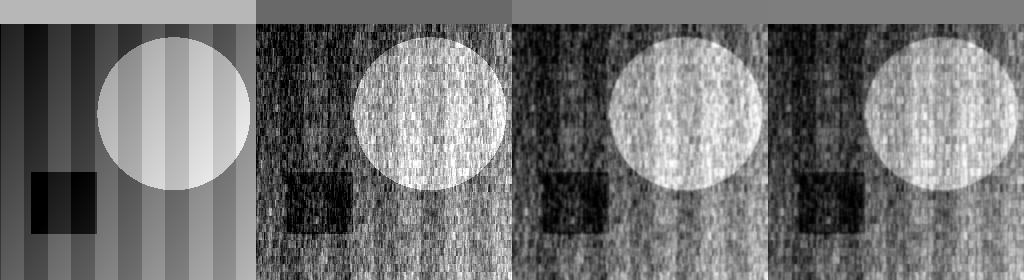
\includegraphics[width=\textwidth]{results/card_demo.png}

  \vspace{0.2cm}
  Left to right: clean image, correlated noisy image, Gaussian baseline,
  CARD-style restoration.
\end{frame}

\begin{frame}{Measured Output}
  \begin{table}
    \centering
    \begin{tabular}{lcc}
      \toprule
      Image & PSNR & SSIM \\
      \midrule
      Correlated noisy & 18.62 & 0.889 \\
      Gaussian baseline & 22.07 & 0.946 \\
      CARD-style restore & 22.39 & 0.949 \\
      \bottomrule
    \end{tabular}
  \end{table}

  \vspace{0.3cm}
  The covariance-aware restoration improves over both the noisy input and the
  Gaussian baseline in this deterministic demonstration.
\end{frame}

\begin{frame}{Difference from the Original Paper}
  \begin{table}
    \centering
    \small
    \begin{tabular}{lll}
      \toprule
      Component & Original CARD & This Project \\
      \midrule
      Restoration engine & DDRM diffusion sampler & Wiener-style denoising \\
      Learned prior & Pretrained diffusion model & Gaussian image prior \\
      Tasks & Denoising, deblurring, SR & Denoising only \\
      Noise data & Synthetic and real CIN-D & Synthetic only \\
      Covariance & Dark frames or synthetic & Hand-designed synthetic \\
      Evaluation & ImageNet, LSUN, CIN-D & One deterministic demo \\
      \bottomrule
    \end{tabular}
  \end{table}
\end{frame}

\begin{frame}{Why This Version Is Useful}
  \begin{itemize}
    \item It runs quickly on CPU.
    \item It has no pretrained model dependency.
    \item The covariance and restoration logic are easy to inspect.
    \item It demonstrates the core insight of CARD:
      \[
        \text{model the noise correlation instead of pretending it is i.i.d.}
      \]
    \item It is suitable for a course presentation and reproducible experiment.
  \end{itemize}
\end{frame}

\begin{frame}{Limitations}
  \begin{itemize}
    \item It is not a faithful implementation of the full diffusion/DDRM method.
    \item It does not use real dark-frame calibration.
    \item It does not evaluate on real camera datasets.
    \item It does not support deblurring or super-resolution.
    \item Its SSIM implementation is a simple global metric, not full local-window SSIM.
  \end{itemize}
\end{frame}

\begin{frame}{Conclusion}
  CARD shows that correlated sensor noise should be handled explicitly.

  \vspace{0.4cm}
  This project preserves the central image-processing concept:
  \begin{itemize}
    \item estimate or define a covariance matrix;
    \item use it to color and whiten noise;
    \item restore in a covariance-aware representation;
    \item compare with a method that ignores correlation.
  \end{itemize}

  \vspace{0.3cm}
  The result is a small, reproducible implementation suitable for explaining
  the method before moving to the full diffusion-based version.
\end{frame}

\end{document}
